%!TEX program = xelatex
\documentclass[11pt,article,oneside]{memoir}
\usepackage{org-preamble-xelatex}
\DisemulatePackage{setspace}
\usepackage{setspace}
\usepackage{titling}
\setlength{\droptitle}{-12em}
% \input{vc}


\usepackage{graphicx}
% We will generate all images so they have a width \maxwidth. This means
% that they will get their normal width if they fit onto the page, but
% are scaled down if they would overflow the margins.
\makeatletter
\def\maxwidth{\ifdim\Gin@nat@width>\linewidth\linewidth
\else\Gin@nat@width\fi}
\makeatother
\let\Oldincludegraphics\includegraphics
\renewcommand{\includegraphics}[1]{\Oldincludegraphics[width=\maxwidth]{#1}}

\title{The Early Spread of Mass Media Increases the Probability of Civil War: A
Research Note}

%\author{}

\author{\Large Justin Murphy\vspace{0.05in} \newline\normalsize\emph{University of Southampton} \newline\footnotesize \url{j.murphy@soton.ac.uk}\vspace*{0.2in}\newline }

%\author{Justin Murphy (University of Southampton)}

\date{}


\begin{document}  
\setkeys{Gin}{width=1\textwidth} 	
\setromanfont[Mapping=tex-text,Numbers=OldStyle]{Georgia} 
\setsansfont[Mapping=tex-text]{Gill Sans} 
\setmonofont[Mapping=tex-text,Scale=0.8]{Consolas}
\chapterstyle{article-jmrphy}
\pagestyle{kjh}

\singlespacing


\maketitle



\vspace{-4ex}
\begin{abstract}

\noindent A recent article in \emph{International Organization} suggests that by
enhancing the soft power of states, the spread of mass media decreases
the probability of civil war onset. This research note contributes an
improvement to the logic of that argument (internal consistency) and
demonstrates a substantively different and improved accounting of the
empirical relationship between mass media and civil war (internal and
external validity). Mass media density decreases the likelihood of civil
war only after the treshold at which it constitutes a mass
communications system; before that threshold, year-to-year increases in
mass media density significantly increase the likelihood of civil war.

\end{abstract}

\newpage


\onehalfspacing

\subsection{Intro}\label{intro}

\begin{figure}[htbp]
\centering
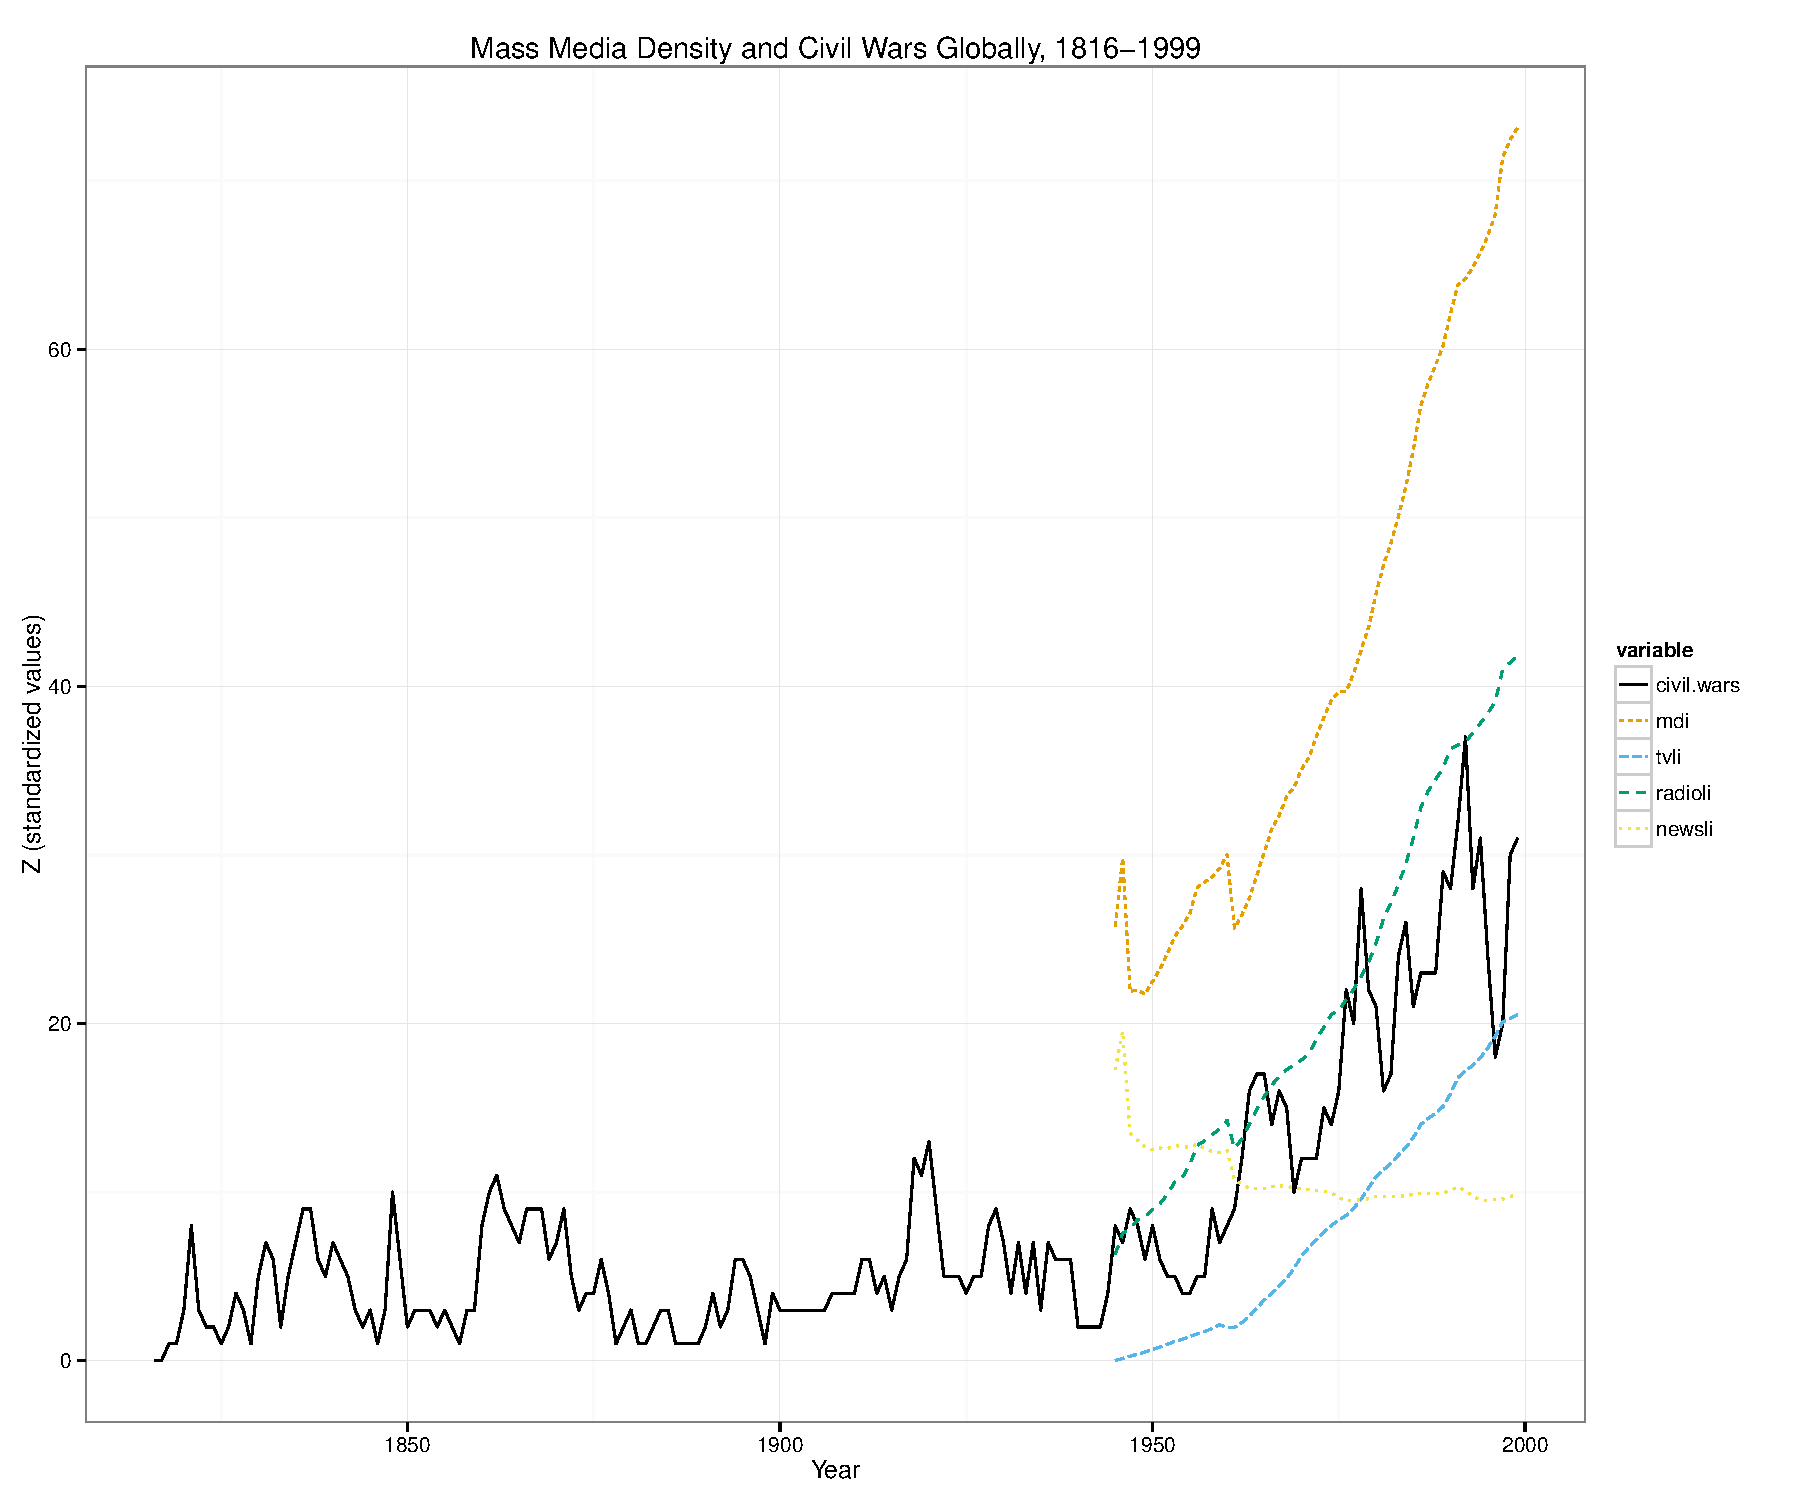
\includegraphics{figure/globalplot.pdf}
\caption{Mass Media Density and Civil Wars Globally, 1816-1999}
\end{figure}

\subsection{Why Mass Media Density is Supposed to Decrease the
Likelihood of Civil
War}\label{why-mass-media-density-is-supposed-to-decrease-the-likelihood-of-civil-war}

In a recent issue of \emph{International Organization}, Camber Warren
argues that the spread of mass media technologies throughout a
particular country decreases the probability of observing civil war
because mass media technologies increase state strength and therefore
deter insurgencies. The reason that technologies such as televisions,
radios, and newspapers enhance the state's strength is because they
increase the state's normative influence and therefore its power to
induce loyalty from citizens. More specifically, mass media technologies
increase this ``soft power'' of the state in two ways.

First, mass media technologies lower the costs of communication in
general, for states as well as insurgents. Second, however,mass media
technologies increase the normative influence of the state in particular
because of economies of scale which are unique to the production of
normative influence. Because a media message achieves a larger effect on
receivers who believe the message was widely disseminated, the
production of normative influence through mass media brings increasing
marginal returns for each additional unit of effort, as each additional
recipient receiving the message increases the effect of the message on
the rest of the receivers. Because the state is inherently a
larger-scale producer of symbolic content than potential insurgent
groups, Warren argues, higher levels of mass media will be associated
with normatively stronger states and therefore lower probabilities of
observing civil war.

Grounding this theoretical model in the tradition of figures such as
Karl Deutsche and Benedict Anderson who first diagnosed the role of mass
media in the rise of modern nationalism, as well as contemporary
experimental research on mass-media messaging, Warren's theory stresses
the unique effects of mass communications relative to small-scale
interpersonal communications. Using state-level data for a large panel
of countries from 1945 to 1999, Warren demonstrates that, after
controlling for other predictors of civil war, mass media density
(televisions, radios, and newspapers per person) is associated with more
than a tenfold decrease in the likelihood of observing civil war in a
particular country-year.

\subsection{A Critique}\label{a-critique}

If higher levels of mass media density decrease the likelihood of civil
war, it is extremely puzzling that in modern history, the international
system's most rapid and widespread proliferation of mass media density
has coincided with its most dramatic increases in civil war. If mass
media density decreases the likelihood of civil war as strongly and
robustly as Warren argues, then why has the global proliferation of mass
media since 1945 had no appreciable effect in pacifying the global
prevalence of civil war?

The first shortcoming of Warren's argument is that, while there should
be increasing marginal returns to the production of normative influence
in the context of \emph{mass communications,} there should not be a
linear, one-to-one relationship between a country's mass media density
and its capacity for mass communications. When only a very small
proportion of the population has access to mass media technologies,
those technologies do not imply the presence of a mass communications
system at merely low levels; they imply a country which still
categorically lacks the infrastructural capacity for properly mass
communications.\footnote{Of course, there is no way to know \emph{a
  priori} how many people need access to mass media technologies before
  they constitute a mass public network and therefore the categorical
  presence of a mass communications system. In any event, the question
  is pursued empirically below. At this stage, it suffices simply to
  note the contention that very low levels of mass media density do not
  reflect the positive presence of a mass communications capacity.} If
only a very small proportion of a population has access to television,
radio, or a newspaper, recipients of mass media messaging will know that
the vast majority of others will not be affected by the message. Thus,
within the subset of countries characterized by very low levels of media
density, the normative influence of messages delivered by mass media
technologies should not be enhanced by increasing marginal returns as
these are contingent on the recipient believing the message to be
\emph{widely} spread.

Mass media density only captures the reach of mass communications within
a particular country beyond the threshold at which mass media
technologies are sufficiently widespread to effectively consititute a
mass public network.\footnote{I assume throughout that mass media
  typically first appears within countries at very low levels relative
  to the population (low media density). I also assume throughout that,
  despite variable rates of change and short-run decreases, media
  density has a long-run tendency to increase. In other words, I assume
  that the dynamics of media density are non-stationary and trend
  upward. The Levin-Lin-Chu (2002) and Im-Pesaran-Shin (2003) tests for
  stationarity in panel data fail to reject the null hypothesis that
  media density is non-stationary (p = 0.75 and p = 0.1, respectively).
  See the Appendix for details.}

The second shortcoming is that if the level of mass media \emph{in
general} increases state strength as Warren argues, then for this very
reason, the \emph{first appearance and early growth} of mass media
within a country should increase the utility of controlling the state
relative to other means of merely influencing it. Especially given that
mass media density is non-stationary and trends upward in every country
in which it has been introduced, the first appearance of mass media
technology should increase the incentives of opposition groups to risk
insurgency before the development of a mass communications system
significantly increases the power of the incumbent and decreaes the
power of opposition groups outside the state. Additionally, the closer a
country's mass media density is to the threshold at which it will
constitute a capacity for mass communcations, the more attractive it
will be for opposition groups outside the state to gain control of the
state. It is increasingly urgent as the state becomes nearer to
consolidating its normative domination via mass communications and
therefore significantly less vulnerable to insurgency; also, the closer
the country is to the threshold the less time will a successful
insurgency be vulnerable to yet another insurgency before it
consolidates its own normative consolidation via mass communications.
Thus, if it is true that increasing mass media density makes state power
increasingly safe from insurgency, then before media density crosses the
threshold of constituting mass communications power, \emph{each
increase} in mass media density should further increase the payoffs to
violent insurgency.

\subsection{A Modified Theory of Mass Media Technology and Civil
War}\label{a-modified-theory-of-mass-media-technology-and-civil-war}

Based on the implications of the previous section, this research note
advances a crucially modified theory of the relationship between mass
media technology and civil war: while high levels of mass media density
should indeed decrease the likelihood of civil war by increasing state
power and deterring insurgents, for this very reason the
\emph{introduction and early growth} of mass media density within a
country should \emph{increase} rather than decrease the likelihood of
civil war. Precisely because a capacity for mass communications
increases state power and becomes a robust deterrent against insurgents,
but low levels of mass media density do not yet constitute that power,
year-to-year increases in mass media density up to a certain threshold
should be positively associated with civil war onset.\footnote{It stands
  to reason that the same logic characterizes the incentives of
  incumbents, as each increase in mass media density up to that
  threshold also increases the utility of defeating insurgencies
  relative to stepping down or sharing power, thus further predicting
  civil war onsets. Yet the calculus of incumbents is likely more
  complicated given that under certain conditions it could be preferable
  to share the state's new mass communications power rather than risk
  losing it. At present, I focus on the calculus of insurgents and leave
  the calculus of incumbents to future research.} It is only beyond that
threshold that Warren's finding of a negative relationship between mass
media density and civil war should hold.

To test whether this modified theory is preferable to Warren's
attractively parsimonious theory, I pursue a strategy of increasing
causal leverage relative to the original analyses (G King, Keohane, and
Verba 1994, 30). A first strategy to increase causal leverage is to
deduce from the modified theory additional observable implications
exclusive to the modified theory, which expose the modified theory to
new opportunities for falsification.

Thus, I deduce three distinct observable implications of the modified
theory which either contradict the original theory or are not implied by
the original theory. If the modified theory is correct, then each of the
following should be true:

\textbf{Observable implication 1:} There should exist a threshold of
mass media density below which year-to-year increases in mass media
density \emph{increase} the probability of civil war. This implication
flows directly from the logical critique of the original theory: If a
system of mass communications constitutes a significant increase in the
soft power of states and makes insurgency significantly more difficult,
then every increase in mass media density (the dynamics of which are
non-stationary and upward-trending) incentivizes insurgency without yet
increasing the risks.

\textbf{Observable implication 2:} Because newspaper and television
production are subject to more significant economies of scale and higher
fixed costs than radio production, increases in newspaper and television
density should be more strongly associated with civil war onset than
increases in radio density before the threshold of mass
communications.\footnote{While these technologies are equally subject to
  economies of scale in their ``symbolic''" production (each additional
  message communicated decreases the cost of convincing another person
  of the message), here I refer to traditional or material economies of
  scale in the concrete production processes.} While each newspaper and
television production requires subsantial technological and logistic
investment the average costs of which decrease with scale, radio
productions are far less technologically and logistically costly and
therefore do not benefit as much from scale. The substantive political
implication of this difference is evidenced by historically and
geographically widespread examples of anti-state radio projects but far
fewer instances of anti-state television or newspapers with mass
audiences. While semi-illegal ``underground'' newspapers have been
historically and geographically widespread, the significant economies of
scale in newspaper production are such that they are almost always
limited to very limited circulation. After the threshold of mass
communications, the state's soft power increases more from mass
newspaper and television audiences than mass radio audiences, because
the economics of radio make mass radio audiences comparatively more
contestable by resource-poor challengers. Note that year-to-year
increases in radio density should still be positively associated with
the likelihood of civil war as radio production is still subject to
material and symbolic economies of scale which nonetheless will
privilege the state after the threshold of mass communications is
crossed, however less significant they are in comparison to newspaper
and television production.

\textbf{Observable implication 3:} Given that mass media technologies
increased markedly after World War II as measured at the international
level, year-to-year increases in mass media density at the international
level should be associated with increases in the quantity of civil wars
at the international level. On the contrary, if the general pacification
theory is correct, then a greater density of mass media around the world
should be associated with a greater number of civil war onsets. Note,
however, that the war-before-peace theory is consistent with the general
pacification theory in the expectation that mass media density in the
long run has a pacifying effect on the likelihood of civil war onset,
after controlling for the bellicose implications of year-to-year
changes.

\subsection{Data and Method}\label{data-and-method}

This section outlines the data, method, and overall analytical strategy
designed to weigh the general pacification theory (levels of mass media
density monotonically decrease the likehlihood of civil war onset) with
the war-before-peace theory (early increases in mass media density
increase the likelihood of civil war before levels of mass media density
decrease it in the long-run). As already discussed, the first feature of
the research strategy was to deduce distinct observable implications of
the new, competing hypothesis, at multiple levels of analysis, which
contradict or are not implied by the original hypothesis. This section
first details the data and methodological strategy for testing the first
two observable implications, and then considers separately the data and
methodological strategy for testing the third implication at the
international level.

The first two stages of analysis for the first two observable
implications use the replication data from Warren (2014), a panel
dataset of country-level variables covering 0 countries over a maximum
of 55 years in the period 1945-1999. As the variables used in the
present analyses follow the original analyses as exactly as possible,
for the sake of consistency and comparison, readers may consult the
original article for a more detailed discussion of the data. Briefly,
the dependent variable in all analyses is \emph{CIVIL WAR ONSET}, which
takes a value of 1 for all country-years in which a civil war begins and
zero otherwise. Civil wars are defined, following Sambanis (2004), as
any armed challenge to state sovereignty with explicit political
objectives, local recruits, and more than 500 deaths in the first year
or more than 1,000 deaths within the first three years. The main
indepdendent variable is \emph{MDI,} which captures overall mass media
density, or the total number of newspapers, televisions, and radios per
100 people. \emph{NEWSPAPER}, \emph{TV}, and \emph{RADIO} reflect the
number of each particular technology per 100 people. A battery of
control variables which are believed to be associated with civil war
onset include the following. \emph{OIL EXPORTER} takes a value of 1 if
greater than one-third of a country's total export revenus are from
fossil fuels. \emph{DEMOCRACY} is the traditional measure from the
well-known Polity IV data set, on a scale from 1-21.
\emph{DEMOCRACY\^{}2} is the square \emph{DEMOCRACY}, to control for the
possibility of non-linear effects. \emph{PEACE YEARS} counts the number
of years since a previous civil war, and a natural cubic spline of peace
years to control for temporal dependence. Finally, \emph{GDP PER
CAPITA}, \emph{ETHNIC FRACTIONALIZATION}, \emph{RELIGIOUS
FRACTIONALIZATION}, and logarithms for \emph{LAND AREA},
\emph{MOUNTAINOUS TERRAIN}, and \emph{POPULATION} complete the main
battery of controls dictated by previous research and employed in the
original analyses. Also following the original analyses, all independent
variables are lagged by one year.

Because observable implication 1 posits a threshold or tipping-point
beyond which the hypothesized effect of mass media changes direction, it
raises the question of how to test for the presence of such a threshold.
The typical procedure for testing the presence of curvilinear effects is
to include in regression analysis a polynomial of the independent
variable of interest; if both the linear term and the polynomial are
differently signed and significant, it is taken as evidence of a
curvilinear effect. The first problem with this convention is that it
does not conveniently inform us about the thresholds for the independent
variable's heterogenous effects, and indeed is typically used as a
substitute for having to do so. More importantly, however, parametric
estimates can fail to detect important curvilinear effects (Fr{ö}lich
2006). On the other hand, nonparametric regressions are significantly
less theoretical and less parsimonious and therefore less valuable for
theory testing.

To balance these trade-offs, analysis begins with a combination of
classic graphical analysis and non-parametric regression to test for the
presence of a threshold at which the effect of mass media density
changes, and then traditional parametric regressions will provide
additional tests and more useful estimates of effect sizes. Graphical
analysis is used to explore several features of the distributions of
mass media density and civil war relevant to understanding their
relationship, discussion of which is postponed until the analysis in the
following section. To statistically test whether mass media density has
a non-linear effect on civil war onset, and to gain further insight into
the threshold at which mass media density constitutes a mass
communications system, a semi-parametric Generalized Additive Model
(GAM) is estimated such that the effect of mass media density is
estimated via nonparametric smooth but all other predictors are
estimated traditionally. Estimation via non-parametric smooth basically
allows for the maximum-likelihood estimate of a traditional logistic
regression to inductively identify curvature in the relationship between
the independent and dependent variable; the smoothness of the curves is
determined by penalized regression splines which are themselves
estimated to maximize likelihood. While the GAM model with
non-parametric smoothing is a well-established tool for testing
non-linear hypotheses, it is not readily interpretable and inferentially
problematic precisely because it lacks a parameter (coefficient) which
could straightforwardly represent a hypothesized effect. Thus, a simple
analysis of variance (ANOVA) is used to test whether a non-linear fit of
mass media density better explains variation in civil war onset than a
linear fit; and graphical visualization of the smooth terms will be used
to further understand the threshold at which mass media density
constitutes a mass communications system. If a non-linear fit of mass
media density is superior to a linear fit and the graphical inspections
reveal a non-trivial subset of civil war onsets increasing in mass media
below an identifiable threshold at which mass media density is robustly
associated with decreasing probability of civil war, then we will
consider observable implication 1 to be tentatively confirmed and the
subsequent analyses will be informed by these preliminary analyses.

To further explore observable implication 1 and test oservable
implication 2, the analysis replicates a baseline model from Warren's
original analysis (2014) and tests whether the pacification effect is
observed even within the subset of country-years characterized by mass
media density levels below the threshold (if any) identified in the
first analyses. If observable implication 1 is shown to be consistent
with the data in the first stage of analyses, it will be expected that
the pacification effect of mass media density will not hold within the
subset of country-years below the threshold at which it constitutes a
mass communications system. On the contrary, the expectation advanced by
the war-before-peace theory is that year-to-year increases in mass media
density will \emph{increase} the likelihood of civil war onset rather
than decrease it. Observable implication 2, which predicts that the
bellicose effects of mass media density should be greatest for newspaper
and television density compared to radio density, is examined by
additional regression analyses which disaggregate the indepedent
variable of mass media density into its component parts. Observable
implication 2 will be affirmed if the coefficients for newspaper and
television density are greater than and statistically distinguishable
from the coefficients for radio density.

Observable implication 3 seeks causal leverage from a level of analysis
distinct from the level at which the original theory was tested
(country-level). Additionally, observable implication 3 permits
examination of a substantially expanded historical range because for
many of the key variables data are available beginning from the early
nineteenth century. For the dependent variable, the Correlates of War
data provide a comprehensive record of all intra-state wars since 1816.
The Polity IV measure of democracy, discussed above, covers many
countries as far back as 1800 and is commonly used for
international-level estimates. For the other key determinant of civil
war onset, GDP per capita, the Maddison Project provides widely-used
estimates for all countries as far back as possible, in many cases
extending well before 1800. Finally, while no general measure of mass
media density is available before 1945, I exploit a pecularity of
television diffusion to reliably and substantially extend its
time-series. Because the international mean for television density is
zero in the earliest year available (1945) and the time-series of
television density is an integrated (unit-root) process which trends
upward, the international mean for television density in every year
prior to 1945 is highly likely to be zero. Thus, I construct an
historically-extended international-level variable for \emph{TV}
equivalent to the one discussed above but which takes a zero for all
years prior to 1945.

To test observable implication 3, I estimate a series of regressions
using the negative binomial distribution for count data, where the
dependent variable is the total count of civil wars in the international
system. While the theoretical issues of time-series modeling of count
data are not negligible, a lagged dependent variable is conventiently
interpretable as a growth rate and adequately controls for
autocorrelation given an integrated dependent variable (BRANDT). To
increase robustness, I consider two versions of the dependent variable.
A first model considers the count of onsets, as in the main analyses,
and a second model considers the number of intra-state wars taking place
(civil war prevalance).

One drawback to this strategy is that several of the other control
variables in the main regressions are not available for such a long
historical period and their omission could lead to biased or spurious
estimates. Luckily, there are several good reasons why the threat of
omitted variable bias is outweighed by the leverage gained by testing
these hypotheses from an international-level and elongated time-series
perspective. First, the variables related to physical geography such as
\emph{OIL EXPORTER}, \emph{LAND AREA} and \emph{MOUNTAINOUS TERRAIN} are
unlikely to vary appreciably because, while in principle they can vary
from changes in the number or size of states, they refer to quantities
which are ultimately fixed at the international level. Second, while
variables such as \emph{RELIGIOUS FRACTIONALIZATION} and \emph{ETHNIC
FRACTIONALIZATION} are likely to have varied since 1816, a far greater
proportion of their variance is likely to be cross-sectional and
therefore irrelevant to modeling civil wars at the international level.
Third, if one re-estimates the original models from the 1945-1999 period
with only the democracy variables and GDP per capita as the only control
variables, the estimates are not substantially different than the full
models with all controls, suggesting that time-series analysis excluding
these variables is still a credible strategy for hypothesis testing. The
fourth key reason why these risks of omitted variable bias are not
prohibitive is that the theoretical and subsantive gains of extending
the original sample to a long-run historical time-series analysis are
great: theoretically it is necessary because the arbitrarily truncated
nature of the original sample does not contain enough information
regarding the key relevant comparison (namely, the difference between
positive and zero mass media density), substantively because the most
politically salient and puzzling stylized fact about civil war is its
far greater prevalence in the period 1945-1999 \emph{compared} to the
previous period of modern world history.

Another drawback to this strategy is that considering only television
density apart from newspaper and radio density may fail to capture mass
media density in general. However, first, television density is highly
correlated with mass media density and disaggregated regressions in the
original analyses also show that television density has strong and
robust effects in the same, expected direction of mass media density.
Second, because television, with newspapers, is subject to greater
economies of scale than radio and is therefore more likely to be
pacifying, it should therefore be a relatively harder test of the
war-before-peace hypothesis than mass media density in general. If mass
media density truly has a monotonic pacifiying effect on the likelihood
of civil war rather than the non-linear effect hypothesized here, then a
long-run time-series analysis of television density should be more
likely to suggest monotonic pacification than mass media density in
general. If the war-before-peace implication is observed for television
density, it would be stronger evidence of the hypothesis than would be a
fuller measure of mass media density.

\section{Analysis}\label{analysis}

\subsection{Graphical analysis}\label{graphical-analysis}

To gain a better sense of the bivariate relationship between mass media
density and civil war onset, while keeping the distributions in
perspective, Figure 2 displays four violin plots.\footnote{The violin
  plot is a relatively new but simple graphical device similar to the
  traditional boxplot but with a density trace (Hintze and Nelson 1998;
  Kastellec and Leoni 2007).} The violin plots on the left display the
distribution of mass media density for all country-years in which there
is no civil war onset, while the violin plots on the left display the
same distribution for all country-years in which there is a civil war
onset. The violin plots in the top half of the figure are scaled by the
total count of cases for all country-years whereas the plots in the
bottom half are scaled with respect to the count of cases within each
distribution. Each plot contains three points which indicate the 25th
percentile, median, and 75th percentile within each distribution. These
plots illustrate three important facts about the distributions of civil
war onset and mass media density in this sample of countries between
1945-1999.

\clearpage
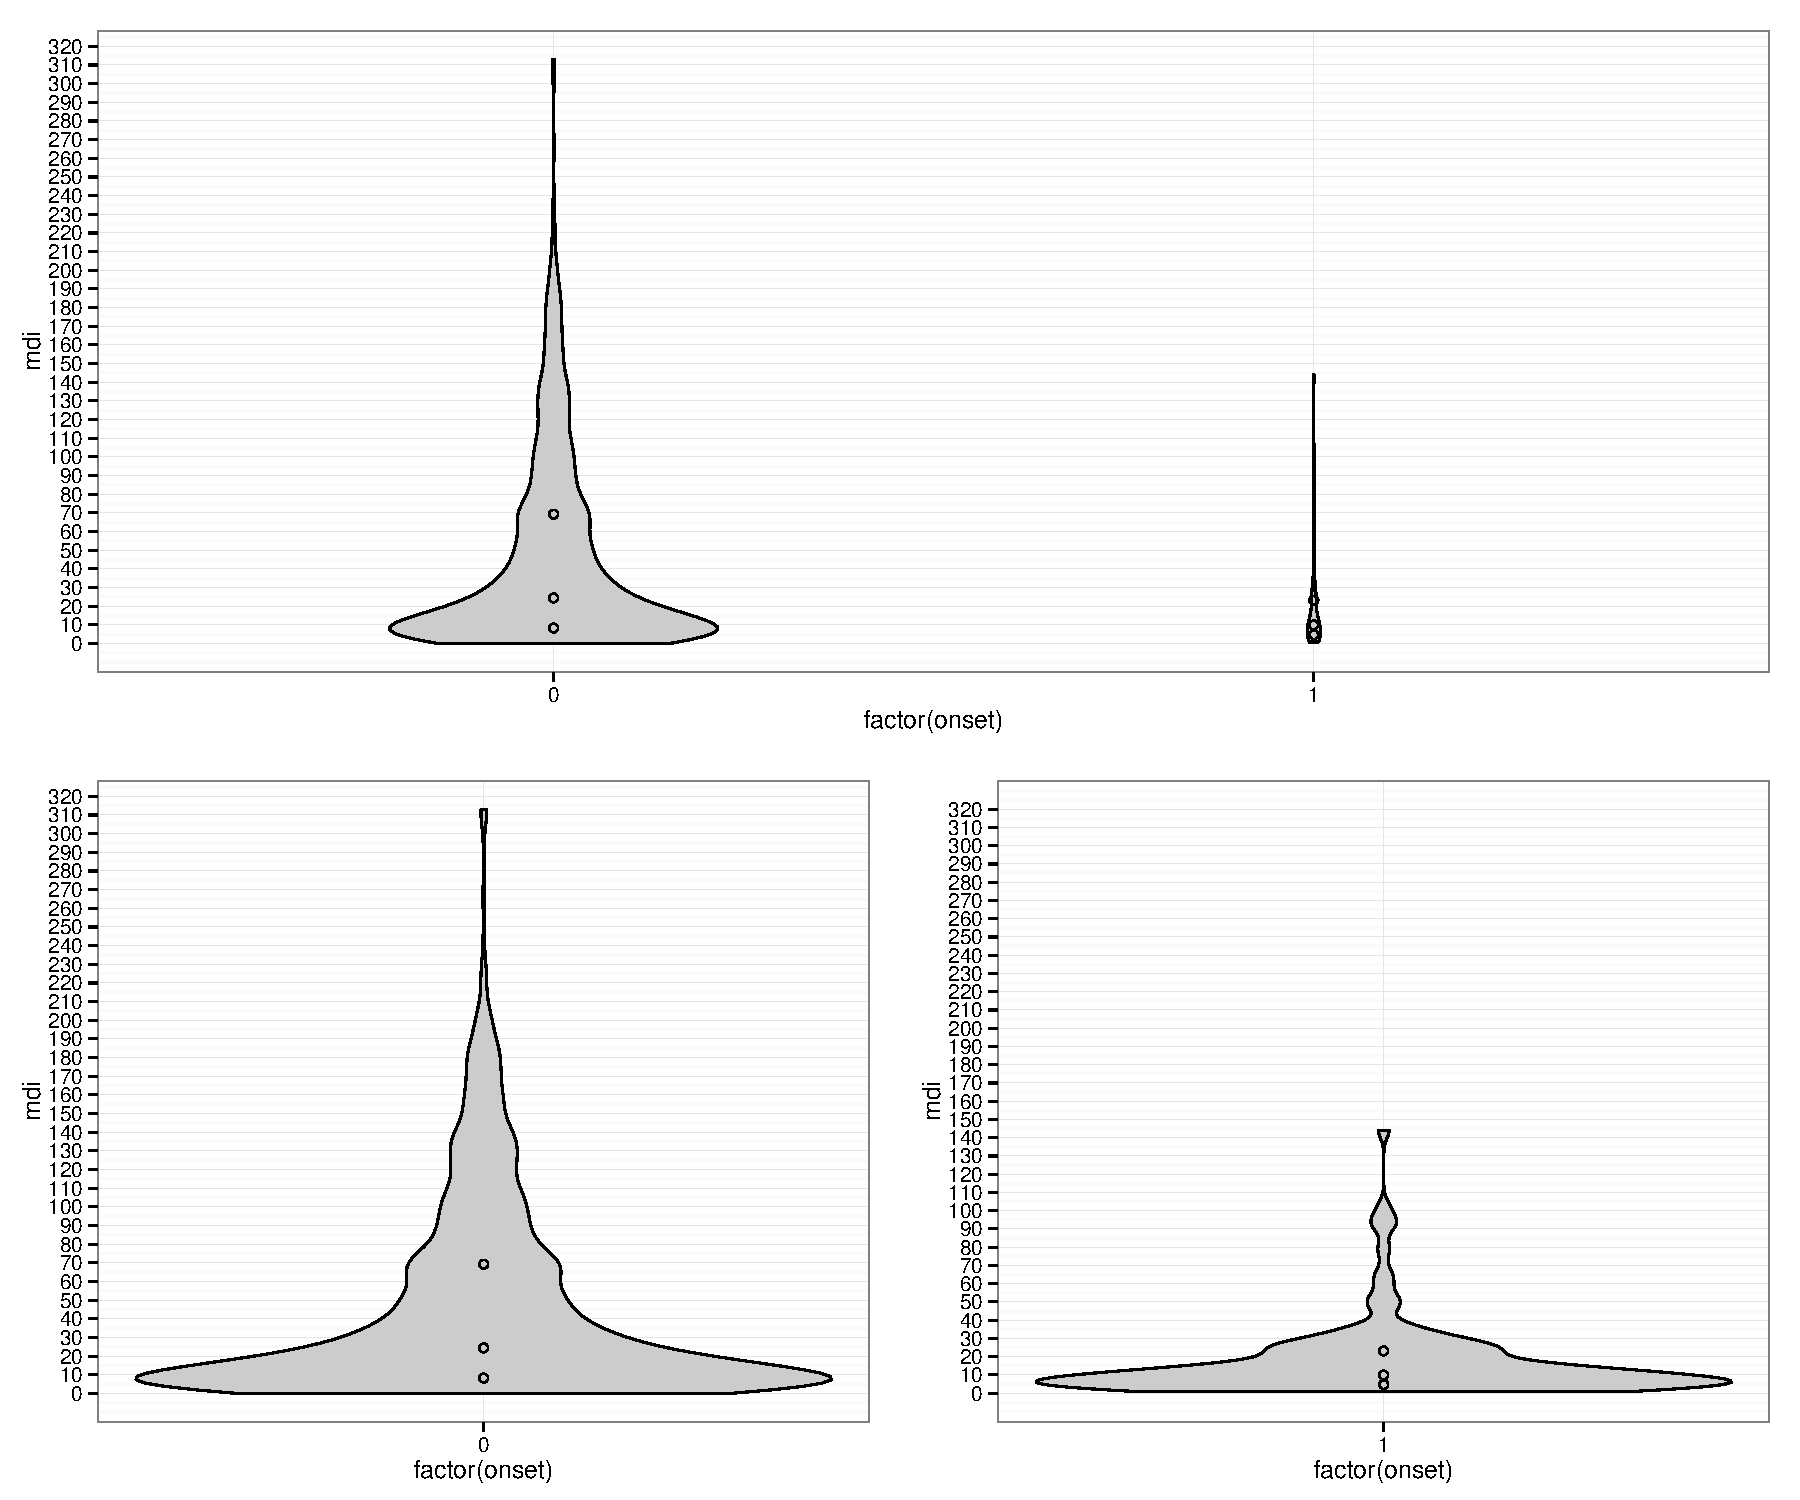
\includegraphics{figure/violinplot.pdf} \clearpage

First, these distributions challenge Warren's key rationale for
questioning the prior belief that mass media plays a causal role in
generating civil war onsets. Warren argues that those cases in which
mass media are known to have played a significant role in civil
war--cases such as Yugoslavia and Rwanda in the early 1990s (MDIs of
40.5 and 6.3, respectively)--``unrepresentative cases\ldots{}
characterized by unusual levels of mass media weakness'' (Warren 2014,
132). Warren argues that because analysts have effectively selected
these cases on the dependent variable, they ``observe mass communication
behavior only in those countries that are experiencing the outbreak of
large-scale civil conflict''(Warren 2014, 132). The implication is that
the positive association between mass media and civil war established by
previous qualitative research is ``spurious'' (132) and that ``expanding
our focus to the full universe of cases reveals quite a different
picture'' (123).

Illustrating the entire distribution of the full universe of cases,
however, Figure 2 illustrates that cases such as Yugoslavia and Rwanda
are indeed fairly typical country-years in the period 1945-1999. While
it is true that in these cases mass media density is below the global
average \emph{in that year}, these cases bracket the global median of
MDI (37.03) by less than half of one standard deviation (8) on either
side. Thus, some of the well-known cases which illustrate the bellicose
effects of mass media are indeed highly representative of MDI levels
globally in the post-war period until 1999.

Second, if there is a problem of unrepresentativeness it is that the
extreme right-skew of MDI in peaceful country-years likely drives a
disproportionate amount of the negative association between levels of
MDI and civil war. Figure 2 illustrates that no civil war has ever been
observed in any country-year characterized by MDI greater than roughly
150, but that these are highly unrepresentative cases (in the 94\%
percentile). This is important because, as the following stage of
analysis will investigate more thoroughly, it indicates that the actual
relationship between mass media and civil war may be driven by a
minority of cases with uncommonly high values on the independent
variable, leading us to inferences which do not necessarily describe
most cases.

Finally, civil wars are most frequently observed at low but positive
levels of MDI, compared to the zero level. \emph{Prima facie} this is
contrary to what we would expect from the general pacification
hypothesis; if the relationship between MDI and civil war onset is
negative and monotonic, we would expect civil wars to be more frequent
at the zero level of mass media density. Rather, the distribution
suggests the possibility of non-linearity at low levels of mass media
density, precisely as predicted by the war-before-peace hypothesis. Of
course, some third variable could very well account for this apparent
non-linearity in the bivariate relationship. For this reason, the
following section turns to a statistical test of this non-linearity,
controlling for all of the other variables in the original model.

\subsection{Considering Non-Linearity with Semi-Paramtric
Regression}\label{considering-non-linearity-with-semi-paramtric-regression}

To test whether mass media density has a non-linear effect on civil war
onset, this section compares the fit of a baseline logistic regression
replicated from Warren (2014) with an additive semi-parametric
regression model identical in every respect except that the effect of
MDI is estimated with a nonparametric smooth allowing it to vary at
different levels of MDI. Specifically, I estimate the model

\[ Onset_{it} = \alpha + f_1 (LogMDI_{it}) + Controls_{it} \beta  + \varepsilon_i \]

where the partial-regression function $f_1 (\cdot)$ is fit by a
smoothing spline ({[}Fox (2002); Wood:2000jb{]}) and $CONTROLS_{it}$ is
the vector of control variables used in Warren's original models. The
number of smoothing splines is determined by generalized cross
validation as part of the estimation procedure.\footnote{The model was
  estimated using the function \emph{gam} in the \emph{mgcv} package for
  R.}

Figure 3 plots the value of the smooth terms for each level of the
logarithm of MDI, i.e.~the estimated effect of the logarithm of MDI on
the probability of civil war onset across its range. The result is
consistent with the war-before-peace hypothesis: MDI is positively
associated with civil war onset up to a threshold, the estimated effect
slightly increasing up to that threshold, before changing direction and
decreasing monotonically. To determine whether the non-linear fit is
superior to the linear fit, a simple analysis of variance (ANOVA) can be
used to contrast the deviance of each model. Table 3 displays the
results, which suggest that the non-linear fit reduces the deviance by
17.9 and is highly statistically significant.

\begin{figure}[htbp]
\centering
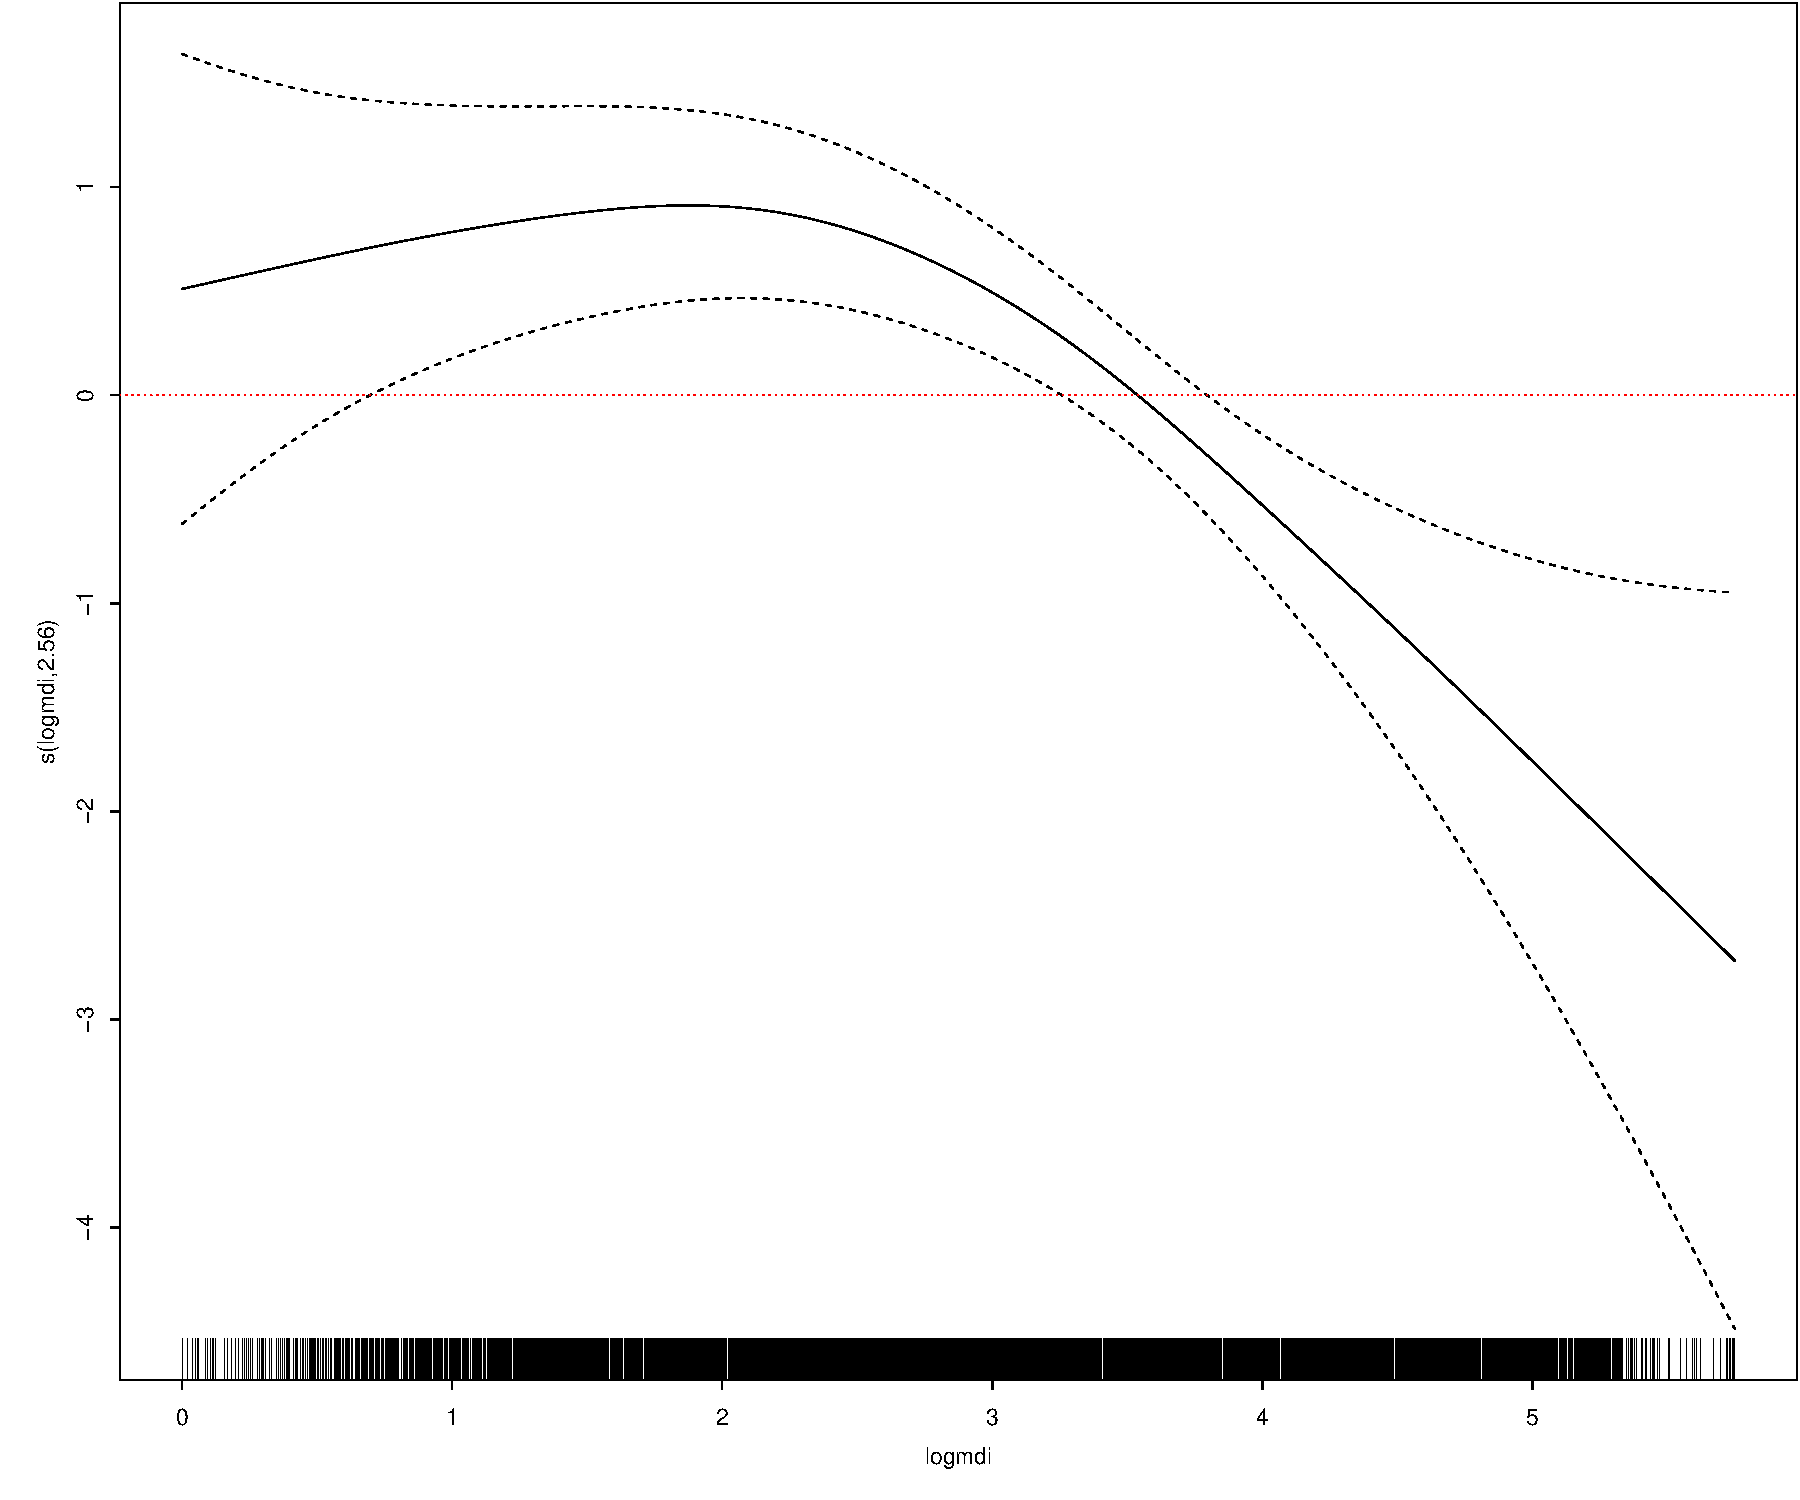
\includegraphics{figure/nonlinear-plot.pdf}
\caption{The Non-Linear Effect of MDI on Civil War Across Levels of MDI}
\end{figure}

\% Table created by stargazer v.5.0 by Marek Hlavac, Harvard University.
E-mail: hlavac at fas.harvard.edu \% Date and time: Wed, Jun 25, 2014 -
19:07:10

\begin{table}[!htbp] \centering 
  \caption{ANOVA Comparing Linear and Non-Linear Effects of MDI on Civil War Onset} 
  \label{} 
\begin{tabular}{@{\extracolsep{5pt}} cccccc} 
\\[-1.8ex]\hline 
\hline \\[-1.8ex] 
 & Resid. Df & Resid. Dev & Df & Deviance & Pr(\textgreater Chi) \\ 
1 & $5,884$ & $1,070.000$ & $$ & $$ & $$ \\ 
2 & $5,882.000$ & $1,052.000$ & $1.600$ & $18.000$ & $0.0001$ \\ 
\hline \\[-1.8ex] 
\end{tabular} 
\end{table}

Table 1 shows coefficients and standard errors from several rare-events
logistic regressions modeling the determinants of civil war
onset.\footnote{Traditional logistic regression estimated by
  maximum-likelihood would likely underestimate the probability of civil
  war onsets because civil wars begin in relatively very few
  country-years (Gary King and Zeng 2001). There are 119 (2.06\%) onsets
  in the full sample and 63 (3.47\%) in the subset of low-MDI country
  years.}

\begin{table}[!htbp] \centering 
  \caption{Early Growth of Media Density Compared to Media Density in General} 
  \label{} 
\footnotesize 
\begin{tabular}{@{\extracolsep{5pt}}lccc} 
\\[-1.8ex]\hline \\[-1.8ex] 
 & Warren & \multicolumn{2}{c}{Low MDI} \\ 
\\[-1.8ex] & (1) & (2) & (3)\\ 
\hline \\[-1.8ex] 
 MDI & $-$2.60$^{***}$ &  &  \\ 
  & (0.71) &  &  \\ 
  $\Delta$MDI &  & 0.43$^{*}$ &  \\ 
  &  & (0.25) &  \\ 
  $\Delta$NEWSPAPER &  &  & 0.26 \\ 
  &  &  & (0.32) \\ 
  $\Delta$RADIO &  &  & 0.30 \\ 
  &  &  & (0.25) \\ 
  $\Delta$TV &  &  & 0.40$^{*}$ \\ 
  &  &  & (0.22) \\ 
  GDP PER CAPITA & $-$0.09 & $-$0.77$^{*}$ & $-$0.78$^{*}$ \\ 
  & (0.36) & (0.40) & (0.40) \\ 
  AREA & $-$0.31 & 0.10 & 0.01 \\ 
  & (0.32) & (0.48) & (0.48) \\ 
  MOUNTAINOUS TERRAIN & 0.45$^{*}$ & 0.34 & 0.37 \\ 
  & (0.24) & (0.39) & (0.40) \\ 
  POPULATION & 0.80$^{***}$ & 0.75$^{*}$ & 0.80$^{*}$ \\ 
  & (0.25) & (0.41) & (0.42) \\ 
  OIL EXPORTER & 0.76$^{***}$ & 1.30$^{***}$ & 1.30$^{***}$ \\ 
  & (0.28) & (0.49) & (0.50) \\ 
  DEMOCRACY & 2.70$^{**}$ & 2.70$^{*}$ & 2.50 \\ 
  & (1.10) & (1.50) & (1.50) \\ 
  DEMOCRACY$^2$ & $-$2.50$^{**}$ & $-$2.20 & $-$2.00 \\ 
  & (1.20) & (1.40) & (1.50) \\ 
  ETHNIC FRACTIONALIZATION & 0.11 & $-$0.43 & $-$0.38 \\ 
  & (0.21) & (0.35) & (0.36) \\ 
  RELIGIOUS FRACTIONALIZATION & 0.60$^{***}$ & 0.40 & 0.47 \\ 
  & (0.23) & (0.36) & (0.36) \\ 
  PEACE YEARS & $-$1.90 & $-$0.55 & $-$0.18 \\ 
  & (2.60) & (2.60) & (2.60) \\ 
  SPLINE 1 & $-$0.55 & 3.30 & 4.50 \\ 
  & (16.00) & (13.00) & (13.00) \\ 
  SPLINE 2 & $-$5.20 & $-$6.00 & $-$6.60 \\ 
  & (18.00) & (15.00) & (15.00) \\ 
  SPLINE 3 & 3.50 & 1.80 & 1.60 \\ 
  & (5.60) & (4.70) & (4.70) \\ 
  CONSTANT & $-$4.50$^{***}$ & $-$3.80$^{***}$ & $-$3.80$^{***}$ \\ 
  & (0.18) & (0.22) & (0.22) \\ 
 \textit{Observations} & 5,899 & 1,445 & 1,445 \\ 
\textit{Log likelihood} & $-$528.00 & $-$182.00 & $-$182.00 \\ 
\textit{Akaike information criterion} & 1,085.00 & 395.00 & 397.00 \\ 
\hline \\[-1.8ex] 
\textit{Notes:} & \multicolumn{3}{l}{$^{***}$p $<$ .01; $^{**}$p $<$ .05; $^{*}$p $<$ .1} \\ 
\end{tabular} 
\end{table}

\clearpage

\begin{figure} 
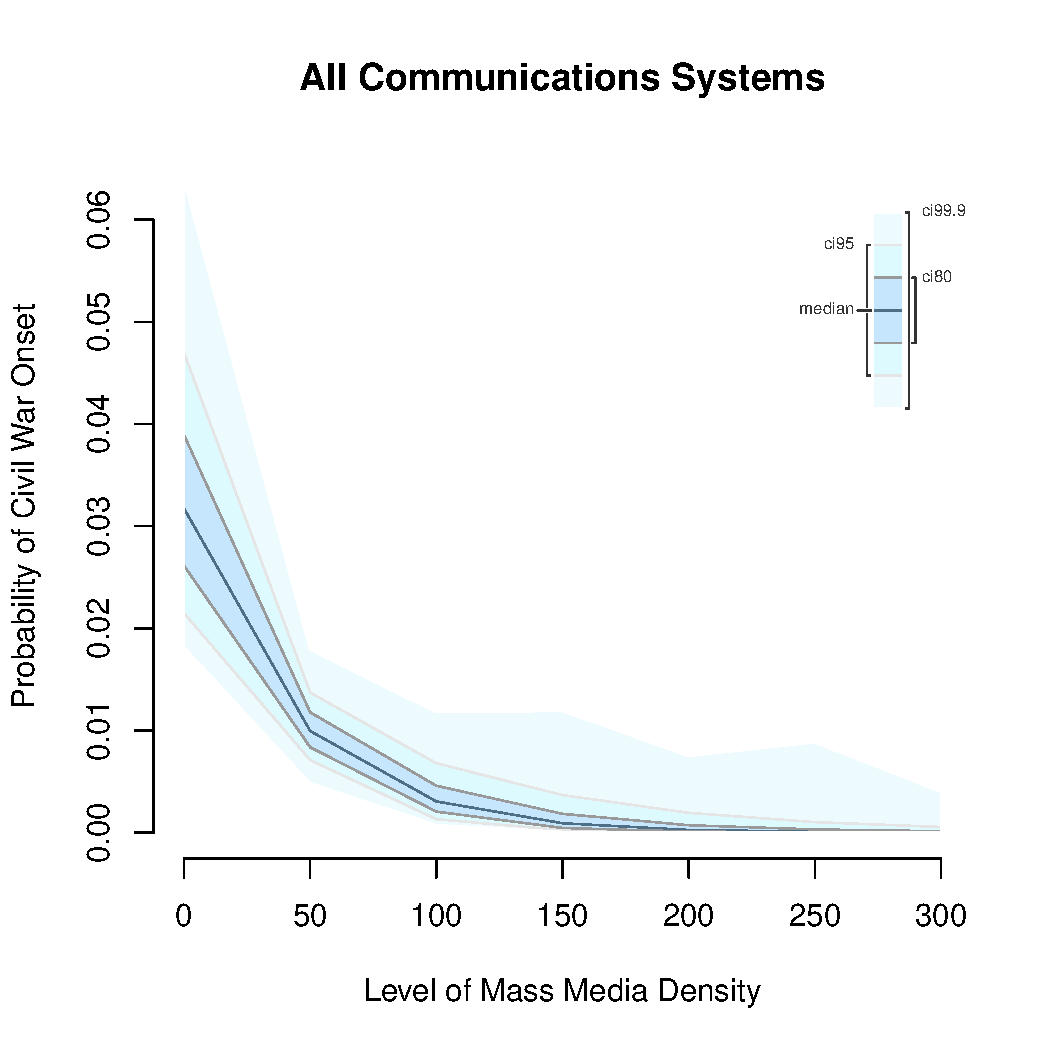
\includegraphics{figure/mdi_effect.pdf} 
\caption{Changes} 
\label{myFigur} 
\end{figure}

\clearpage

\begin{figure} 
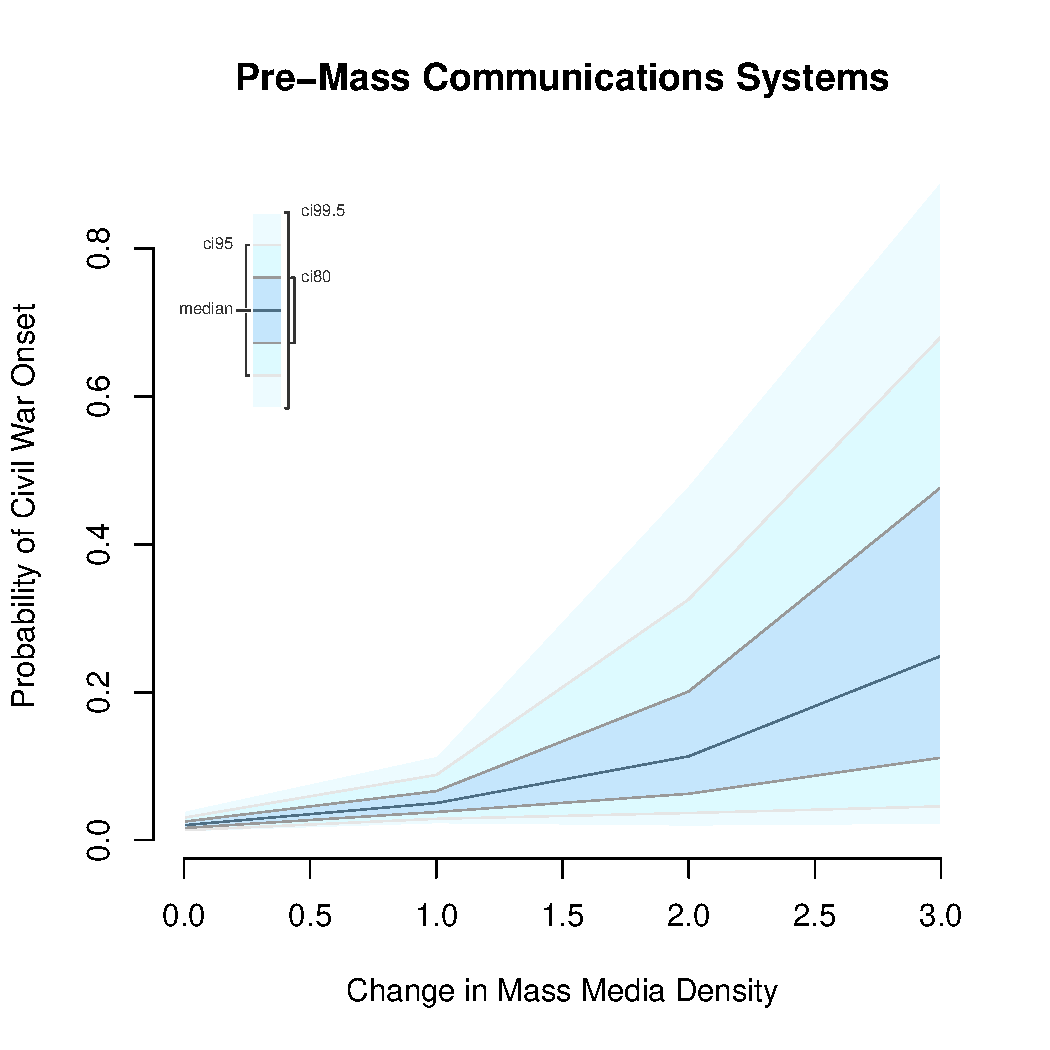
\includegraphics{figure/d_mdi_effect.pdf} 
\caption{Changes} 
\label{myFigz} 
\end{figure}

\begin{figure}[htbp]
\centering
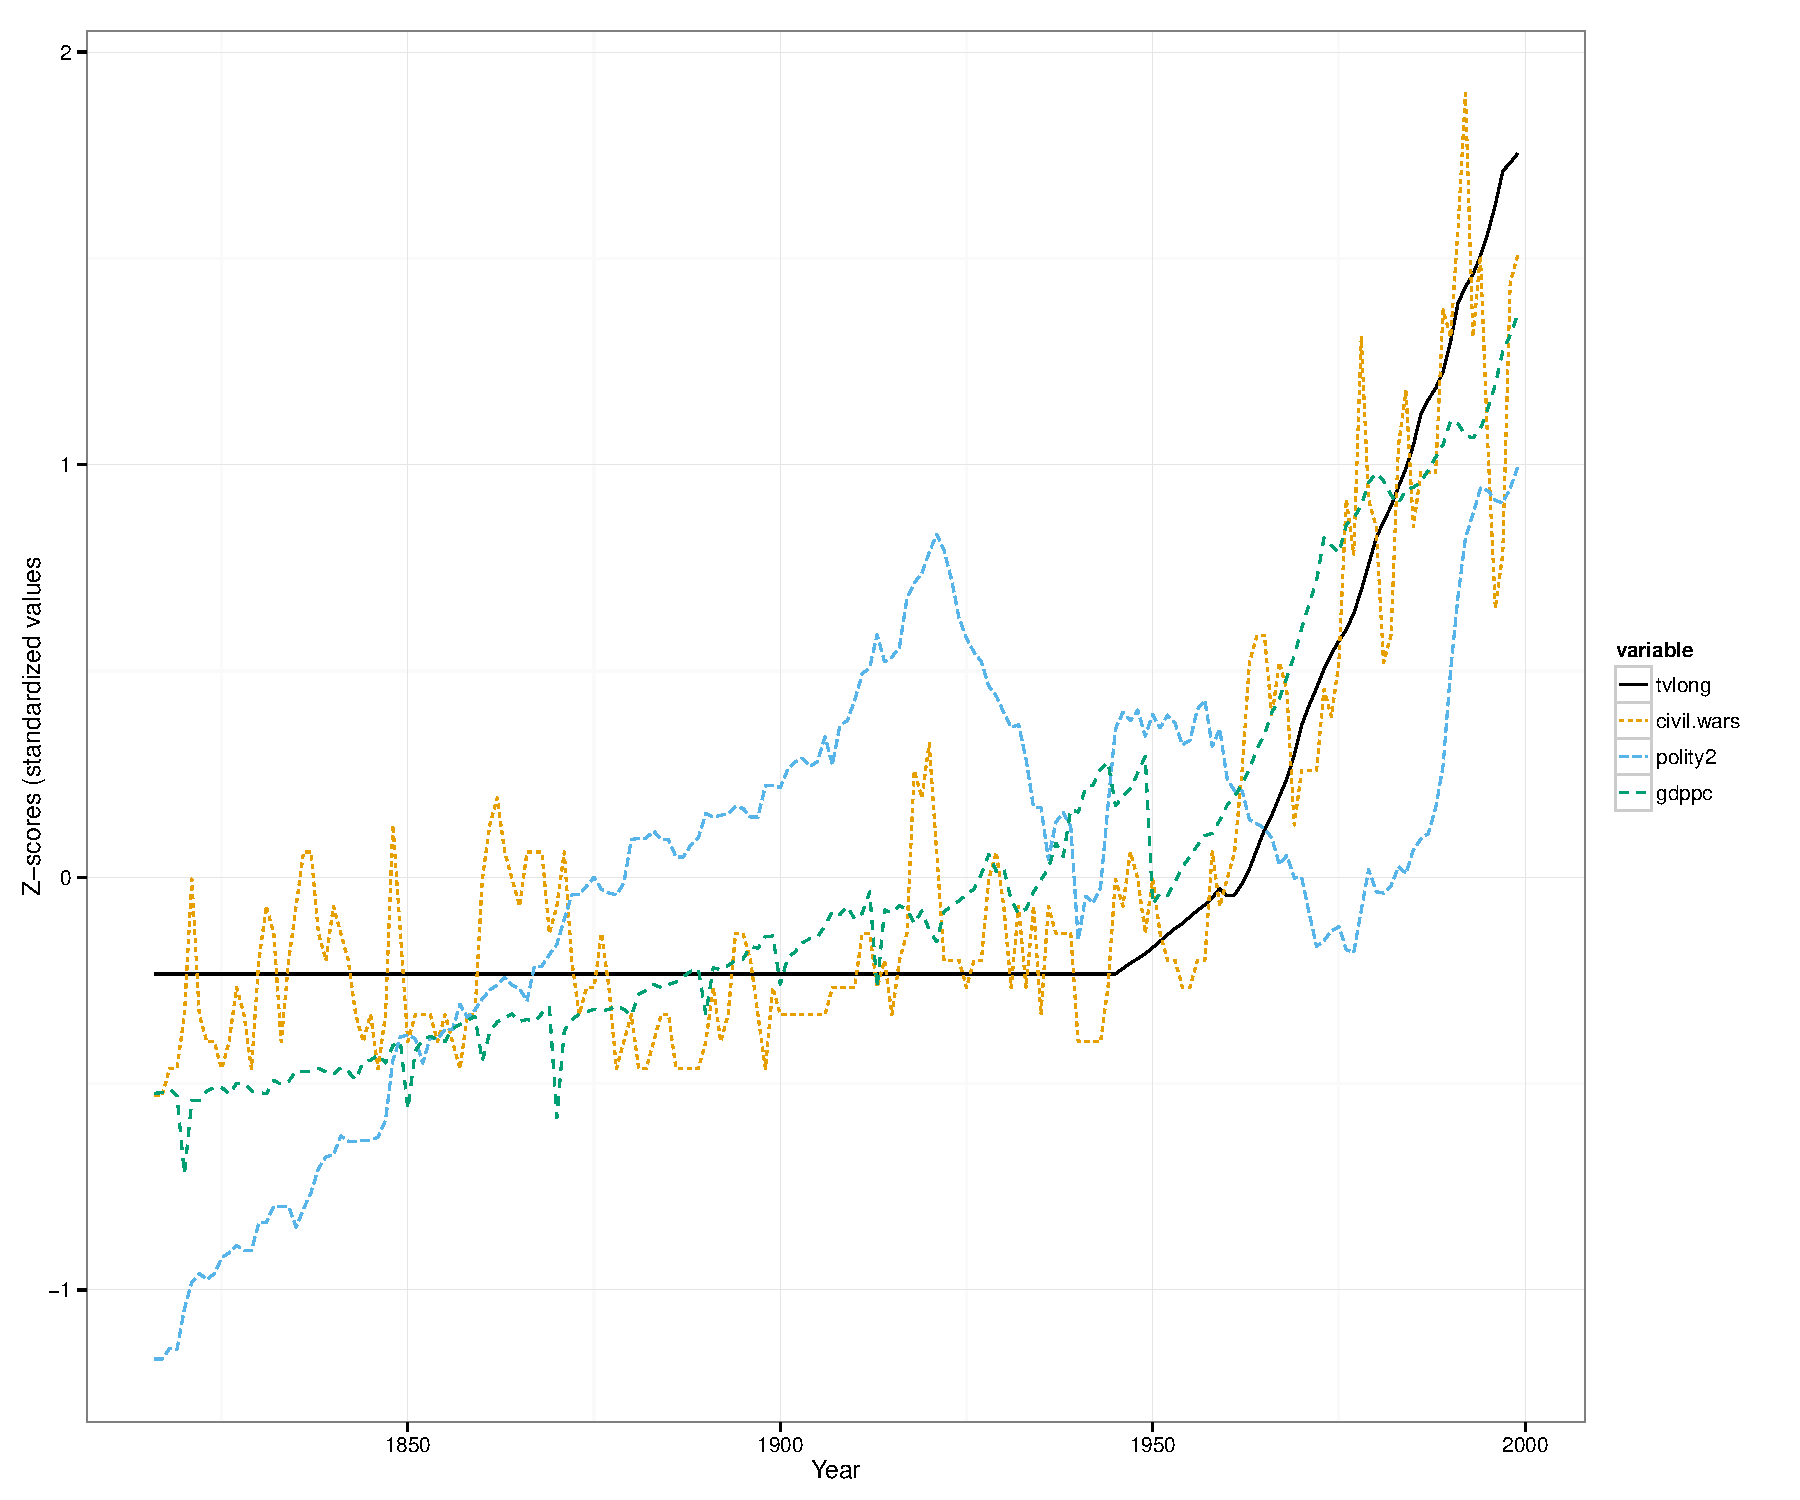
\includegraphics{figure/longrunplot.pdf}
\caption{TV, Democracy, Economic Growth, and Civil Wars Globally,
1816-1999}
\end{figure}

\begin{table}[!htbp] \centering 
  \caption{Historical Regressions} 
  \label{} 
\footnotesize 
\begin{tabular}{@{\extracolsep{5pt}}lccc} 
\\[-1.8ex]\hline \\[-1.8ex] 
\\[-1.8ex] & \multicolumn{3}{c}{onsets} \\ 
\\[-1.8ex] & (1) & (2) & (3)\\ 
\hline \\[-1.8ex] 
 L.TVLONG & $-$0.80$^{***}$ & $-$0.53 & $-$0.40 \\ 
  & (0.30) & (0.35) & (0.34) \\ 
  D.TVLONG & 0.36$^{**}$ & 0.46$^{***}$ & 0.37$^{***}$ \\ 
  & (0.14) & (0.15) & (0.12) \\ 
  L.GDPPC & $-$0.11 & $-$0.06 & 0.80 \\ 
  & (0.50) & (0.55) & (0.53) \\ 
  D.GDPPC & $-$0.01 & $-$0.03 & $-$0.01 \\ 
  & (0.06) & (0.06) & (0.06) \\ 
  L.POLITY2 & 0.20 & 0.86$^{***}$ & 0.75$^{***}$ \\ 
  & (0.16) & (0.22) & (0.24) \\ 
  D.POLITY2 & $-$0.21$^{**}$ & $-$0.21$^{**}$ & $-$0.27$^{***}$ \\ 
  & (0.09) & (0.09) & (0.08) \\ 
  L2.POLITY2 & 0.21 & 0.36$^{*}$ & $-$0.21 \\ 
  & (0.15) & (0.20) & (0.50) \\ 
  CIVIL.WARS & 0.94$^{***}$ & 0.97$^{***}$ & 0.85$^{***}$ \\ 
  & (0.22) & (0.24) & (0.22) \\ 
  L.ONSETS & 0.91$^{***}$ & 0.97$^{***}$ & 0.77$^{***}$ \\ 
  & (0.16) & (0.16) & (0.14) \\ 
  D.ONSETS & 0.16$^{***}$ & 0.17$^{***}$ & 0.14$^{***}$ \\ 
  & (0.02) & (0.02) & (0.02) \\ 
  YEAR & $-$0.09 & $-$0.93$^{*}$ & $-$2.70$^{***}$ \\ 
  & (0.39) & (0.55) & (0.84) \\ 
  WW1 &  & $-$0.10 & 0.17 \\ 
  &  & (0.17) & (0.18) \\ 
  WW2 &  & 0.43$^{**}$ & 0.72$^{***}$ \\ 
  &  & (0.22) & (0.27) \\ 
  COLD &  & $-$0.88$^{***}$ & $-$0.62$^{***}$ \\ 
  &  & (0.20) & (0.20) \\ 
  CONSTANT & 0.53$^{***}$ & 0.56$^{***}$ & 0.66$^{***}$ \\ 
  & (0.04) & (0.08) & (0.22) \\ 
 \textit{Observations} & 182 & 182 & 109 \\ 
\textit{Log likelihood} & $-$260.00 & $-$257.00 & $-$164.00 \\ 
$\theta$ & 45,390.00  (485,212.00) & 45,395.00  (461,838.00) & 67,652.00  (750,223.00) \\ 
\textit{Akaike information criterion} & 544.00 & 544.00 & 358.00 \\ 
\hline \\[-1.8ex] 
\textit{Notes:} & \multicolumn{3}{l}{$^{***}$p $<$ .01; $^{**}$p $<$ .05; $^{*}$p $<$ .1} \\ 
\end{tabular} 
\end{table}

\clearpage

\begin{figure} 
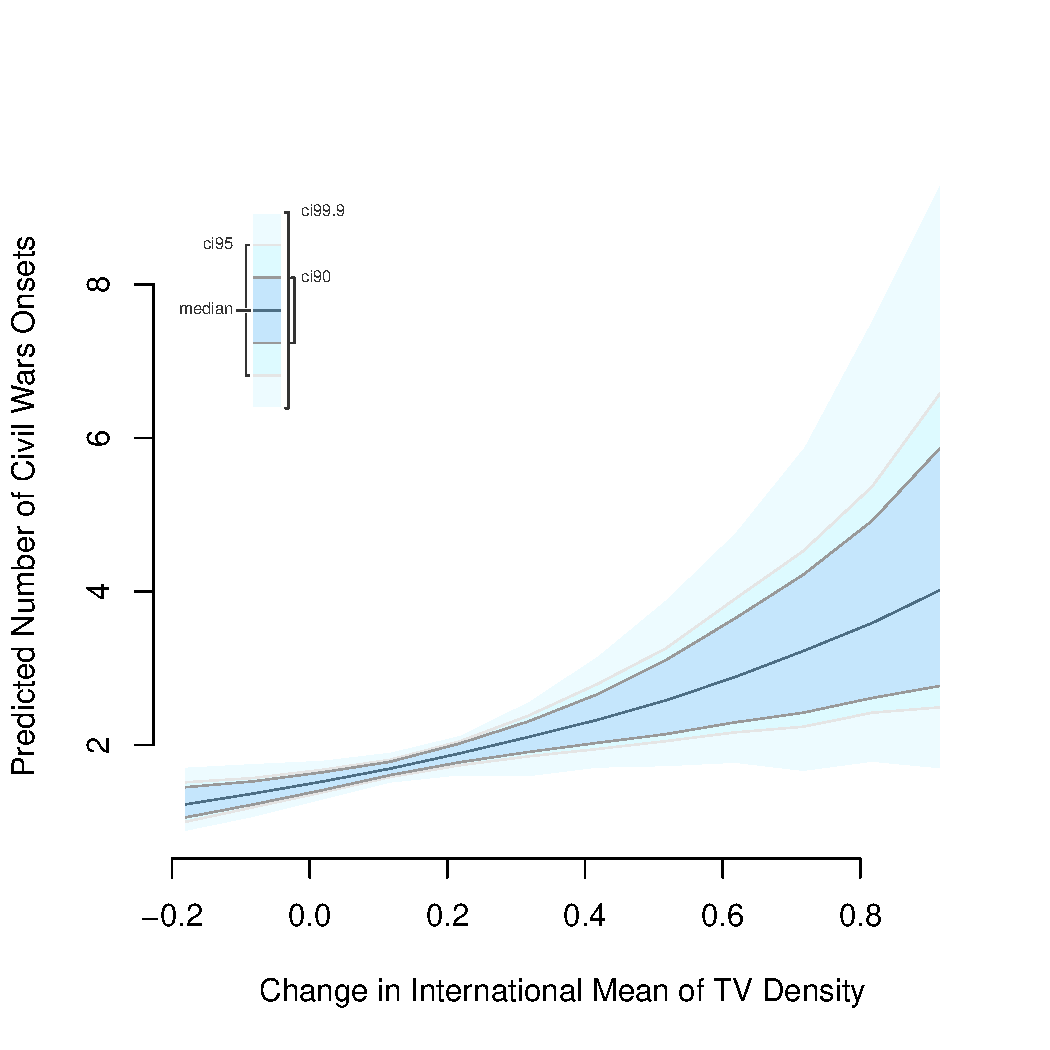
\includegraphics{figure/dtv_effect.pdf} 
\caption{Changes} 
\label{myFigur} 
\end{figure}

\clearpage

\begin{figure}[htbp]
\centering
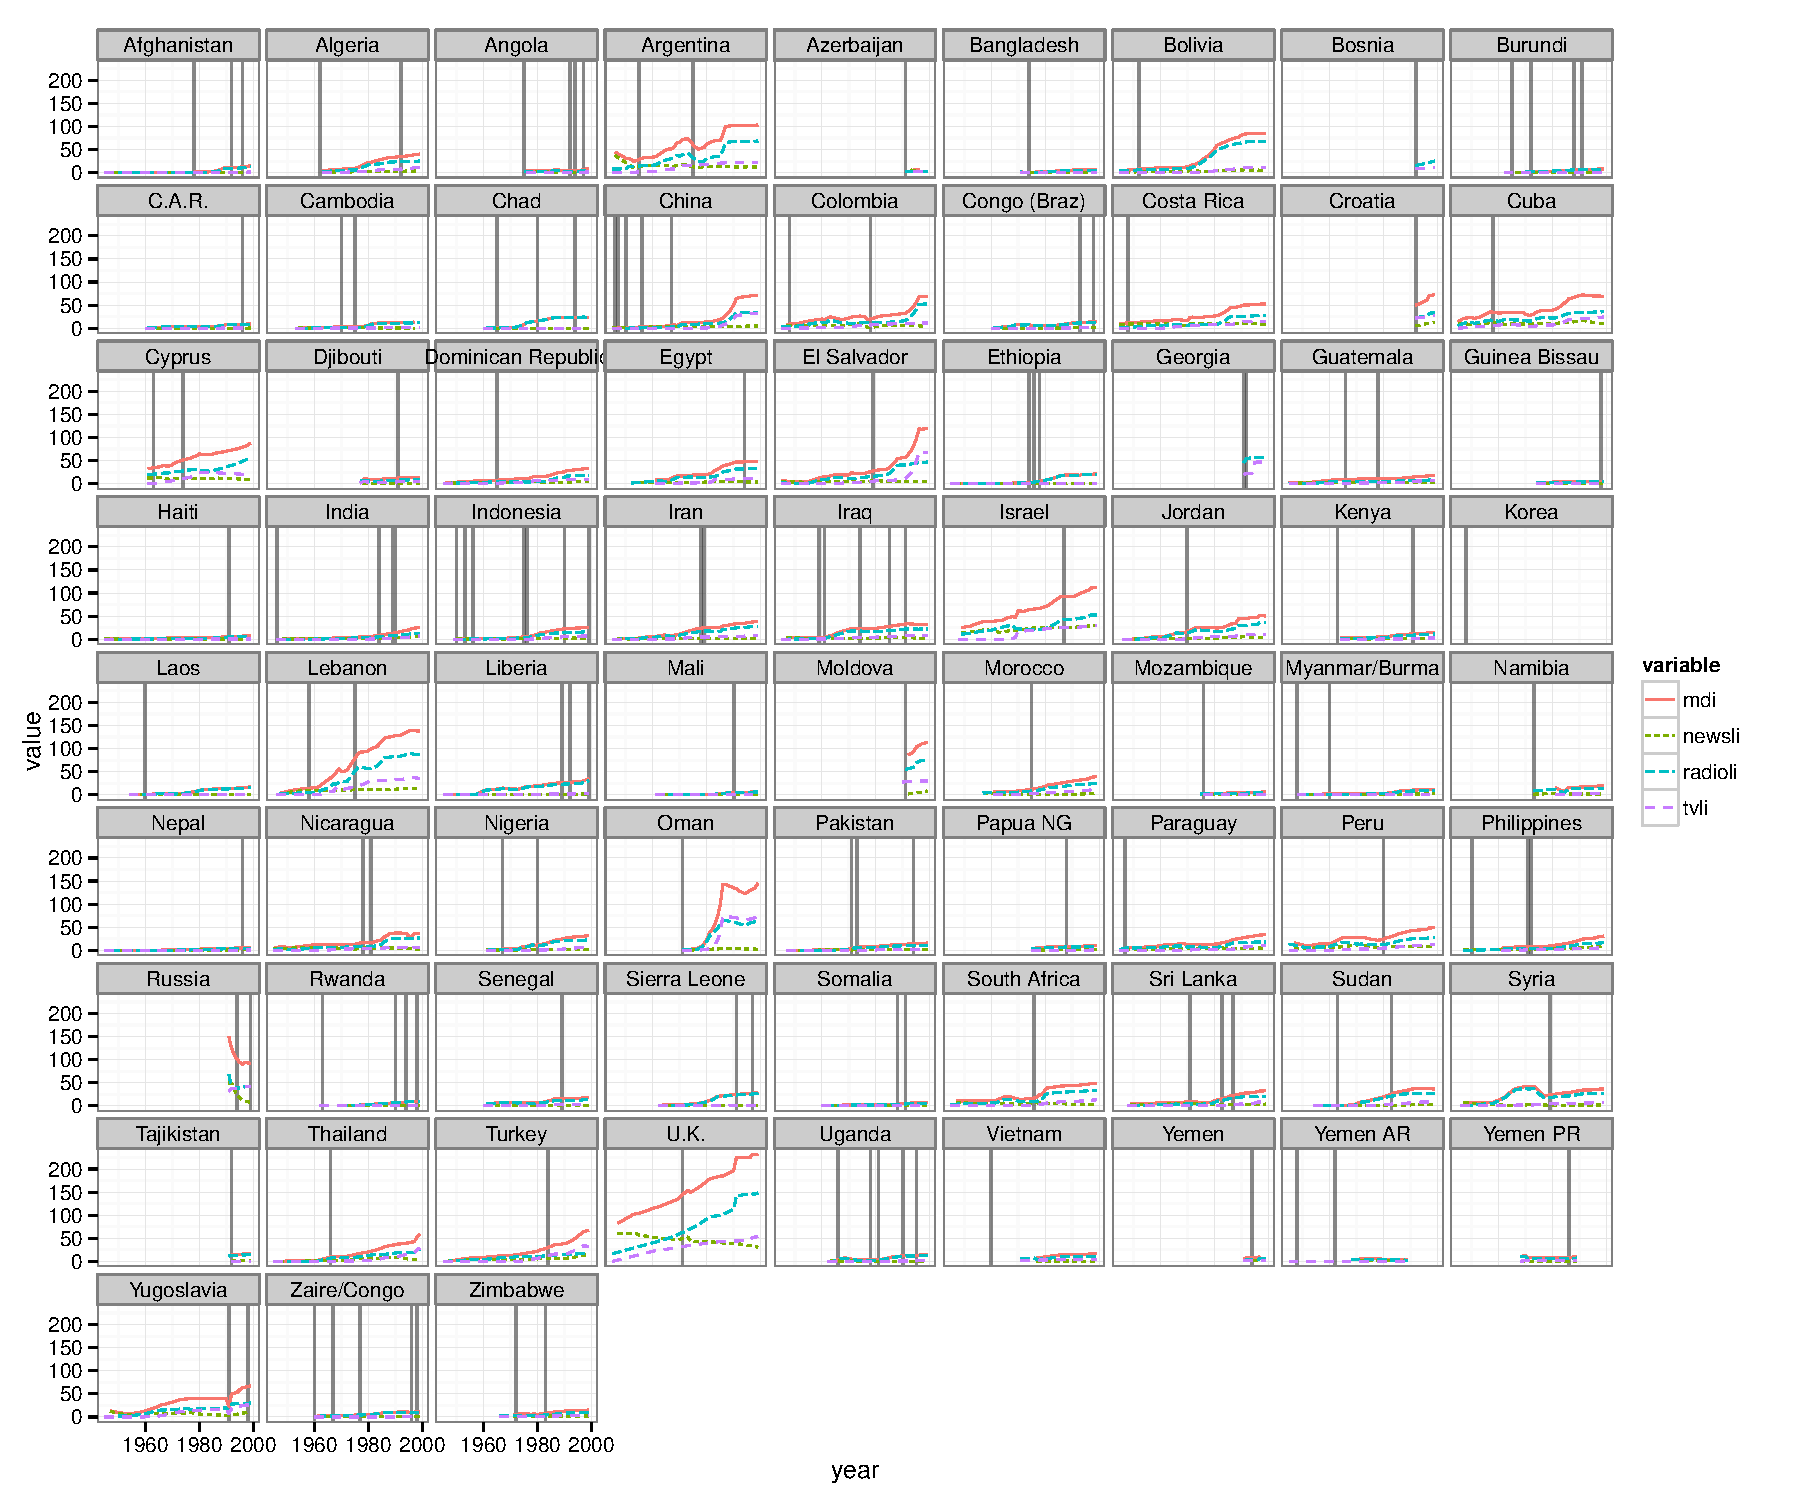
\includegraphics{figure/full_panel_plot.pdf}
\caption{Disaggregated media density and all civil war onsets over time,
by country}
\end{figure}

\section{Conclusion}\label{conclusion}

\section{Appendix}\label{appendix}

The Levin-Lin-Chu statistic is a standard test for the presence of a
unit root, otherwise known as non-stationarity or integration of order
I(1), in a time series variable observed across multiple cross-sectional
units. The Im-Pesaran-Shin test is a ``second generation'' test which is
robust to cross-sectional dependence, common in cross-national panel
data. For each test, the null hypothesis is the presence of a unit root.
Because the tests require balanced panels, they were applied only to the
24 countries with the maximum time-series of 55 years, a subset which
still contains significant variation in geography, income, regime type,
and other factors. Specifically, the countries in this subset are:
Canada, Cuba, Haiti, Dominican Republic, Mexico, Honduras, El Salvador,
Nicaragua, Costa Rica, Uruguay, Ireland, Netherlands, Belgium,
Luxembourg, France, Switzerland, Hungary, Romania, Finland, Sweden,
Norway, Denmark, Afghanistan, China.

\begin{verbatim}
Levin-Lin-Chu Unit-Root Test (ex. var. : Individual Intercepts
and Trend )
\end{verbatim}

data: unit\$mdi z.x1 = -0.32, p-value = 0.7473 alternative hypothesis:
stationarity

\begin{verbatim}
Pesaran's CIPS test for unit roots
\end{verbatim}

data: unit\$mdi CIPS test = -2.1, lag order = 2, p-value = 0.1
alternative hypothesis: Stationarity

\pagebreak   

\section{References}\label{references}

\setlength{\parindent}{-0.2in} \setlength{\leftskip}{0.2in}
\setlength{\parskip}{8pt} \vspace*{-0.2in} \noindent

Fox, John. 2002. ``Nonparametric Regression.'' In \emph{An R and S-Plus
Companion to Applied Regression}, Thousand Oaks, CA.
\url{http://cran.r-project.org/doc/contrib/Fox-Companion/appendix-nonparametric-regression.pdf}.

Fr{ö}lich, Markus. 2006. ``Non-Parametric Regression for Binary
Dependent Variables.'' \emph{Econometrics Journal} 9(3): 511--40.
\url{http://doi.wiley.com/10.1111/j.1368-423X.2006.00196.x}.

Hintze, Jerry L, and Ray D Nelson. 1998. ``Violin Plots: A Box
Plot-Density Trace Synergism.'' \emph{The American Statistician} 52(2):
181--84.
\url{http://www.tandfonline.com/doi/abs/10.1080/00031305.1998.10480559}.

Im, Kyung So, M Hashem Pesaran, and Yongcheol Shin. 2003. ``Testing for
Unit Roots in Heterogeneous Panels.'' \emph{Journal of Econometrics}
115(1): 53--74.
\url{http://linkinghub.elsevier.com/retrieve/pii/S0304407603000927}.

Kastellec, Jonathan P, and Eduardo L Leoni. 2007. ``Using Graphs Instead
of Tables in Political Science.'' \emph{Perspectives on Politics} 5(04):
755--71.
\url{http://journals.cambridge.org.libproxy.temple.edu/action/displayAbstract?aid=1429544}.

King, G, R O Keohane, and S Verba. 1994. \emph{Designing Social Inquiry:
Scientific Inference in Qualitative Research}. Princeton University
Press. \url{http://books.google.com/books?id=A7VFF-JR3b8C}.

King, Gary, and Langche Zeng. 2001. ``Logistic Regression in Rare Events
Data.'' \emph{Political Analysis} 9(2): 137--63.
\url{http://dash.harvard.edu/bitstream/handle/1/4125045/relogit\%20rare\%20events.pdf?s}.

Levin, Andrew, Chien-Fu Lin, and Chia-Shang James Chu. 2002. ``Unit Root
Tests in Panel Data: Asymptotic and Finite-Sample Properties.''
\emph{Journal of Econometrics} 108(1): 1--24.
\url{http://linkinghub.elsevier.com/retrieve/pii/S0304407601000987}.

Sambanis, N. 2004. ``What Is Civil War?: Conceptual and Empirical
Complexities of an Operational Definition.'' \emph{Journal of Conflict
Resolution} 48(6): 814--58.
\url{http://jcr.sagepub.com/cgi/doi/10.1177/0022002704269355}.


\end{document}